\documentclass[10pt,twocolumn]{article}
\usepackage[a4paper,margin=1.6cm,columnsep=0.6cm]{geometry}
\usepackage{amsmath,amssymb}
\usepackage{graphicx}
\usepackage{booktabs}
\usepackage[hidelinks]{hyperref}
\usepackage{titlesec}
\usepackage{enumitem}
\usepackage{caption}
\titlespacing*{\section}{0pt}{5pt}{2pt}
\titlespacing*{\subsection}{0pt}{3pt}{1pt}
\setlist{nosep,leftmargin=*}
\captionsetup{font=small,skip=3pt}
\setlength{\textfloatsep}{6pt}
\setlength{\floatsep}{6pt}
\setlength{\dbltextfloatsep}{6pt}
\setlength{\parskip}{0pt}
\graphicspath{{../results/}}
% generated by scripts/make_report_tables.py -- do not edit by hand
\newcommand{\MainTableRows}{
Policy & Return & Serv.\,\% & Lost & km & Full \\ \midrule
No rebalancing & -413.8 & 87.3 & 366 & 0 & 190 \\
Threshold (default) & -325.3 & 90.4 & 279 & 125 & \textbf{87} \\
Threshold (tuned) & -304.0 & 91.3 & 252 & 136 & 99 \\
\textbf{PPO (ours)} & \textbf{-291.5} & \textbf{91.9} & \textbf{235} & 131 & 119 \\
}
\newcommand{\AblationTableRows}{
Policy & Return & Serv.\,\% & Lost & km & Full \\ \midrule
\textbf{PPO (ours)} & -291.5 & 91.9 & 235 & 131 & 119 \\
\quad no action mask & -305.7 & 91.1 & 257 & 99 & 115 \\
\quad absolute reward (v3) & -335.3 & 89.9 & 290 & 69 & 126 \\
\quad\ \ + amount actions (v2) & -329.7 & 90.0 & 288 & 40 & 137 \\
\quad\ \ + 4N+3 obs, const.\ LR (v1) & -328.4 & 90.3 & 278 & 88 & 131 \\
}
\newcommand{\KmCut}{3}
\newcommand{\LostCutVsNone}{36}
\newcommand{\LostCutVsThr}{7}
\newcommand{\RetPPO}{-291.5}
\newcommand{\RetThr}{-304.0}
\newcommand{\SrPPO}{91.9}
\newcommand{\SrThr}{91.3}
\newcommand{\SrNone}{87.3}
\newcommand{\PairedLost}{16.5}
\newcommand{\PairedLostCI}{11.5}
\newcommand{\PairedLostWins}{19}
\newcommand{\PairedDiff}{+12.5}
\newcommand{\PairedCI}{11.6}
\newcommand{\PairedWins}{18}
\newcommand{\PairedN}{30}
\newcommand{\RobGapHigh}{17.5}
\newcommand{\RobScaleHigh}{1.3}
\newcommand{\RobGapLow}{-5.4}
\newcommand{\RobGapOne}{9.1}
\newcommand{\RobGapTwo}{31.9}

\InputIfFileExists{nomask.tex}{}{}

\title{\vspace{-1.4cm}\textbf{ReBike: Learning Bike-Share Rebalancing with\\Masked PPO on Real Citi Bike Demand}\vspace{-0.3cm}}
\author{Amrit Kumar Yadav (B24CM1008) \quad Raj Kor (B24CM1040)\\
\small GitHub: \url{https://github.com/DeveloperAmrit/rebike}\vspace{-0.4cm}}
\date{}

\begin{document}
\maketitle

\begin{abstract}
\noindent Docking stations that run empty or full turn riders away. We model
truck-based rebalancing as a semi-Markov decision process on a simulator
calibrated from 561k real Citi Bike trips (Jersey City/Hoboken, Jun--Oct 2024),
and train a Proximal Policy Optimization (PPO) agent with invalid-action masking,
target-fill actions and a \emph{counterfactual shadow-day reward} that cancels
demand noise. On 30 held-out October days the agent loses \LostCutVsThr\% fewer trips
than a grid-tuned threshold policy (\LostCutVsNone\% fewer than no rebalancing)
while driving slightly less, and its advantage grows under heavier demand.
\end{abstract}

\section{Problem and Environment}
Commuting makes bike flows strongly directional: residential stations empty in
the morning while business districts fill up. Operators move bikes with trucks,
usually by fixed fill thresholds; optimisation approaches plan overnight or
mid-rush routes from forecasts \cite{omahony2015}. We ask whether an RL policy
can serve more riders per kilometre driven.

\textbf{Demand model.} From the public trip archives \cite{citibike} we keep the $N{=}60$ busiest
stations and estimate, for every hour $h$, Poisson departure rates
$\lambda_{h,i}$, origin--destination probabilities $P_{h,ij}$ and median ride
times $\tau_{ij}$; dock capacities $C_i$ come from the live GBFS feed.
June--September weekdays build the training model, October is held out.

\textbf{Dynamics.} An episode is one weekday (06:00--22:00) simulated in 5-minute
ticks. Rentals at an empty station are \emph{lost}; a rider arriving at a full
station is redirected to the nearest free dock (a \emph{failed dock}). Each day
starts from a \emph{warm start}: one simulated day without a truck and an
overnight crew that fixes 30\% of each station's imbalance, with the fleet at
40\% of docks. A single truck (20 bikes, 18\,km/h, 3\,min handling) acts at
event-driven decision epochs: after an action the clock jumps by the travel
time, while demand keeps being simulated.

\section{RL Formulation}
\textbf{State} $s\in\mathbb{R}^{6N+3}$ ($363$ dims): fill levels $x_i/C_i$;
one-hot truck position; truck load; $\sin/\cos$ of time of day; expected net
inflow over the next hour $(\sum_j\lambda_{h,j}P_{h,ji}-\lambda_{h,i})/C_i$;
bikes in transit arriving within 30\,min; truck travel time to every station;
and the projected fill in one hour (clipped).

\textbf{Action} $a=(j,k)$, $N{\times}6=360$ actions: drive to station $j$ and
bring it to target fill $f_k\in\{0.2,0.35,0.5,0.65,0.8\}$ (moving
$\lfloor f_kC_j\rceil-x_j$ bikes, limited by truck load/space), or drive without
transferring. Target levels mean the same thing at every station, unlike raw
bike counts ($\pm2,5,10$, our first design). Choices that cannot move a bike
(empty truck, station already at target, \dots) are removed with an action
mask \cite{huang2020mask}.

\textbf{Reward.} Policies are scored with the absolute reward
$R_t = -\text{lost}_t - 0.2\,\text{km}_t - 0.25\,\text{failed}_t$ (a km and a
redirected rider as fractions of a lost trip; demand is exogenous, so $-$lost
ranks policies like $+$served). For training we use the \emph{counterfactual}
reward
\begin{equation*}
r_t = R_t - \tilde R_t,\quad \tilde R_t = -\widetilde{\text{lost}}_t - 0.25\,\widetilde{\text{failed}}_t ,
\end{equation*}
where tildes refer to a \emph{shadow day}: the same day, with the same
pre-sampled riders, simulated in lock-step without a truck. $\tilde R_t$ does
not depend on the agent, so the optimal policy is unchanged, but the shared
demand noise cancels (validation std.\ of the return fell from $\approx$80 to
$\approx$35). Pre-sampling riders also gives \emph{common random numbers}: on a
given seed every policy faces identical riders, making all comparisons paired.

\section{Algorithm and Baselines}
We use Maskable PPO \cite{schulman2017ppo,raffin2021sb3}: 8 parallel
environments, 256-step rollouts, batch 512, 10 epochs, $\gamma{=}0.99$,
$\lambda_{\text{GAE}}{=}0.95$, clip 0.2, entropy 0.01, a $256{\times}256$ tanh MLP,
reward normalisation, learning rate $3{\cdot}10^{-4}$ decayed linearly to 10\%,
and 2M environment steps ($\approx$55\,min on 2 CPU cores). The final agent is
the checkpoint with the best return on 30 validation days drawn from the
\emph{training} demand model, so the October test month is never used for model
selection.

\textbf{Baselines.} \emph{No rebalancing}, and a \emph{threshold} policy: with
bikes on board, drive to the station below fill $\ell$ with the best
deficit/distance ratio and fill it to $\theta$; otherwise collect from the
station above $u$. $(\ell,u,\theta)$ is grid-searched on training days (best
$0.15/0.75/0.4$). All policies are scored on the same 30 seeded October days.

\section{Results}
\begin{table}[!t]
\centering\footnotesize
\caption{Held-out October evaluation, mean over 30 days. Lost, km and Full
(failed docks) are per day.}
\label{tab:main}
\setlength{\tabcolsep}{3pt}
\begin{tabular}{lrrrrr}
\toprule
\MainTableRows
\bottomrule
\end{tabular}
\end{table}

PPO achieves the best return (\RetPPO{} vs.\ \RetThr{} for the tuned
threshold; Table~\ref{tab:main}) and service rate (\SrPPO\% vs.\ \SrThr\%;
\SrNone\% without a truck). Paired over the same 30 days it gains
\PairedDiff{}\,$\pm$\,\PairedCI{} return (95\% CI) and saves
\PairedLost{}\,$\pm$\,\PairedLostCI{} trips per day, winning on \PairedLostWins/\PairedN{}
days, while driving \KmCut\% fewer km and moving fewer bikes. Its weak point is
full docks (more redirected riders). Fig.~\ref{fig:hourly} shows where the gain
comes from: the threshold policy only reacts once a station crosses a threshold
and is best at midday, whereas PPO appears to prepare for the evening peak
(using the time and inflow features), losing 25--43\% fewer trips at 17--18\,h.

\begin{figure}[!t]
\centering
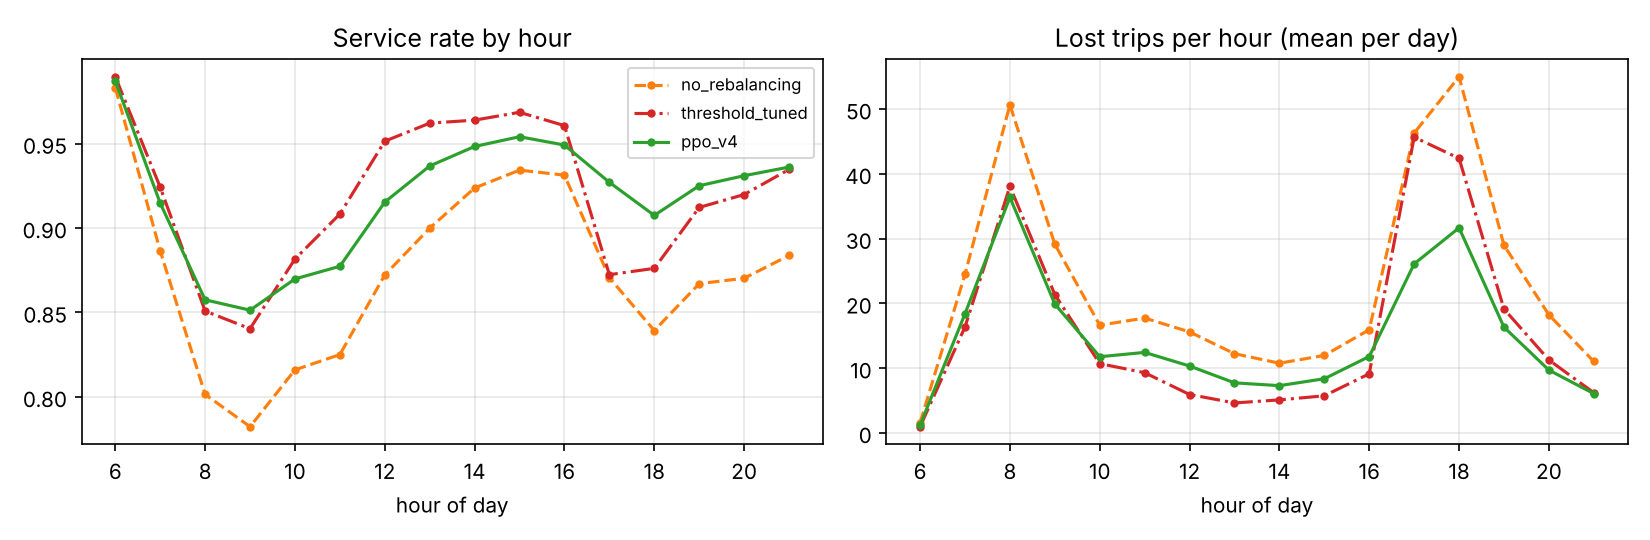
\includegraphics[width=\linewidth]{hourly_service.png}
\caption{Service rate and lost trips by hour of day (October, 30 days).}
\label{fig:hourly}
\end{figure}

\textbf{Ablations} (Table~\ref{tab:ablation}).
Removing the counterfactual reward (v3, same target actions; stopped at 1.25M
steps after plateauing) costs $\approx$44 return and drops PPO below even the
default threshold. Bike-amount actions (v2) and, additionally, the smaller
observation without travel times and constant learning rate (v1) stay at the
same level, and so do their learning curves (Fig.~\ref{fig:curve}). The
counterfactual reward is therefore the decisive ingredient.
\NOMASKTEXT

\begin{table}[!t]
\centering\footnotesize
\caption{Ablations on the same 30 October days.}
\label{tab:ablation}
\setlength{\tabcolsep}{3pt}
\begin{tabular}{lrrrrr}
\toprule
\AblationTableRows
\bottomrule
\end{tabular}
\end{table}

\begin{figure}[!t]
\centering
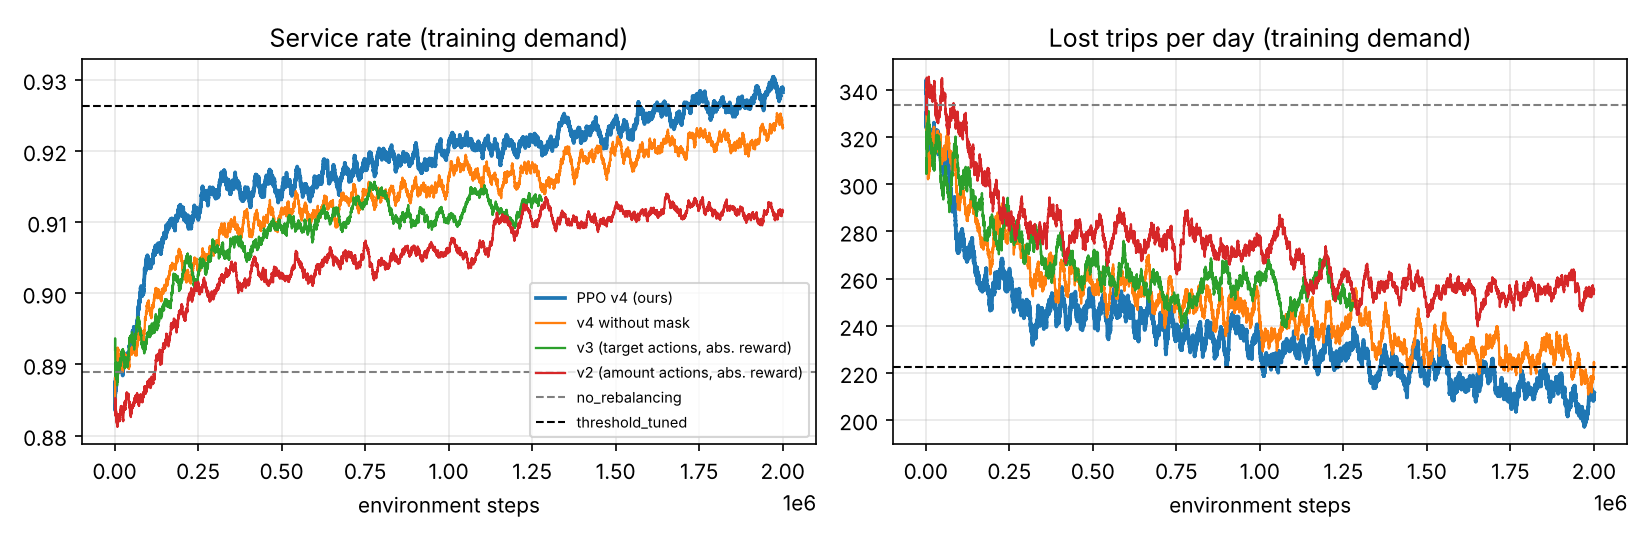
\includegraphics[width=\linewidth]{training_curve.png}
\caption{Learning curves (stochastic training policy, rolling mean over 200
days of training demand); dashed: baselines on training demand.}
\label{fig:curve}
\end{figure}

\begin{figure}[!t]
\centering
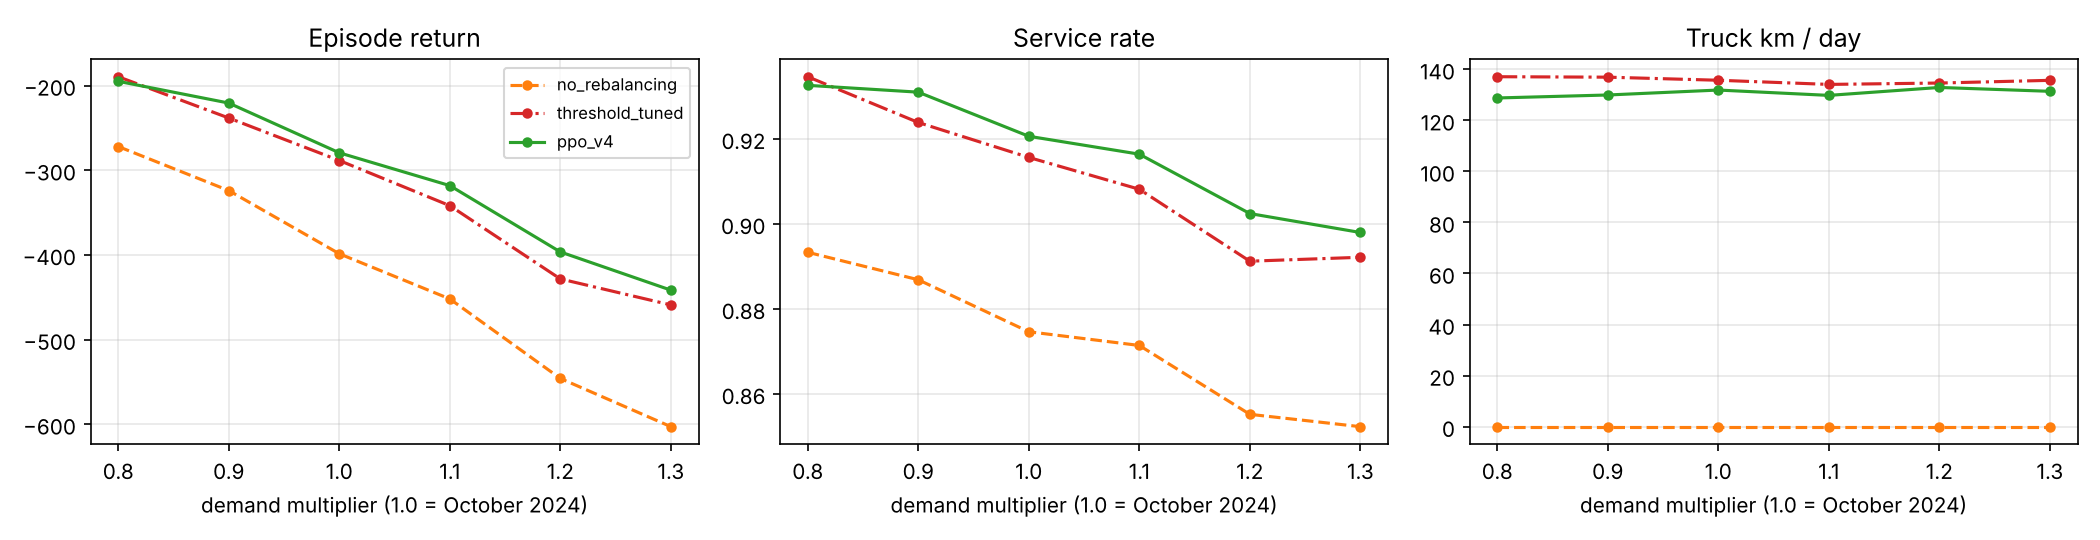
\includegraphics[width=\linewidth]{robustness.png}
\caption{Held-out October days with demand scaled by 0.8--1.3 (15 days each);
agents are not retrained.}
\label{fig:robust}
\end{figure}

\textbf{Robustness} (Fig.~\ref{fig:robust}). Scaling October demand by 0.8--1.3 without retraining,
PPO's return advantage over the tuned threshold grows from \RobGapLow{} at
0.8$\times$ to \RobGapOne{} at 1.0$\times$ and \RobGapTwo{} at 1.2$\times$: the
learned policy matters most when the system is under stress.

\section{Discussion}
A masked PPO agent beats a carefully tuned rule-based policy on unseen days,
but only after two design choices: actions expressed as target fill levels and
a shadow-day reward that removes exogenous demand noise from the learning
signal. The latter is cheap (one extra simulation without a truck) and applies
to any RL problem whose reward is dominated by uncontrollable randomness.
Limitations: a single truck, 60 stations, a simulator without traffic or
weather, and one training seed. The learning curve was still improving at 2M
steps, so longer training, several trucks and dock-blocking penalties are
natural next steps.

{\small
\begin{thebibliography}{9}\setlength{\itemsep}{0pt}
\bibitem{schulman2017ppo} J.~Schulman, F.~Wolski, P.~Dhariwal, A.~Radford, O.~Klimov.
Proximal Policy Optimization Algorithms. arXiv:1707.06347, 2017.
\bibitem{huang2020mask} S.~Huang, S.~Onta\~n\'on. A Closer Look at Invalid Action
Masking in Policy Gradient Algorithms. FLAIRS, 2022 (arXiv:2006.14171).
\bibitem{raffin2021sb3} A.~Raffin et al. Stable-Baselines3: Reliable Reinforcement
Learning Implementations. JMLR 22(268), 2021.
\bibitem{omahony2015} E.~O'Mahony, D.~B.~Shmoys. Data Analysis and Optimization for
(Citi)Bike Sharing. AAAI, 2015.
\bibitem{citibike} Citi Bike System Data. \url{https://citibikenyc.com/system-data}.
\end{thebibliography}}

\end{document}
